\documentclass{whutmod}
\usepackage{metalogo}
\usepackage{float}
\usepackage{subfigure} 
\usepackage{url}
\usepackage{booktabs}
\bibliographystyle{unsrt}
\team{23}
\membera{刘子川}
\joba{编程}
\memberb{程宇}
\jobb{建模}
\memberc{祁成}
\jobc{建模}
\hypersetup{
	colorlinks=true,
	linkcolor=black
}

\title{基于xx模型}
\tihao{1} 

\begin{document}

%\maketitle

	%目录
	\thispagestyle{empty}
	\tableofcontents
	\setcounter{page}{0}                                               
	\newpage	%换页符
	
	\section{问题重述}	
	\subsection{问题背景}
   在物资调运过程中,完成指定点的调运任务是最基本
   的要求,在完成基本的任务之外,往往有更高的追求,比如
   如何使总运费最省?怎样才能使得运输时间最短?如何选
   择运输路径使得运输总距离最短等等。这些更高的追求往
   往是企业期望达到的目标,为了解决这些类似问题,有必
   要对物资调运的过程进行数学模型的建立,以期通过模型
   来理解和分析物资调运的过程,并为其找到解决的方法。
   现以具体的食品调运案例进行分析研究。
    
    某食品公司有19个食品销售点,销售点的地理坐标和每天的需求量见附件。每天凌晨都要从仓库(第20号站点)出发将食品运至每个销售点,运送物品后最终返回仓库。现有运送食品的运输车,每台车每日工作 4小时,运输车重载运费2元/吨公里,并且假定街道方向均平行于坐标轴,任意两站点间都可以通过一次拐弯到达。

	\subsection{问题概述}
    围绕相关附件和条件要求,研究食品运输车在各仓库间的调度方案,依次提出以下问题:
		 
	
	\textbf{问题一:}若只有一辆载重100吨的大型运输车,运输车平均速度为40公里/小时,每个销售点需要用20分钟的时间下货,空载费用0.6元/公里。它送完所有食品并回到仓库,求最少需要时间及其对应的总距离,总运费。
	
	\textbf{问题二:}有一种小型运输车,运输车平均速度为50公里/小时,每个销售点需要用5分钟的时间下货,载重为6吨,空载费用0.4元/公里;要使它们送完所有食品并回到仓库,运输车应如何调度使总体调度效率最高? 
	
	\textbf{问题三:}如果有载重量为4吨、6吨两种运输车,空载费用分别为0.2、0.4元/公里,其他条件均相同,又如何安排车辆数和调度方案。

	
	\section{模型假设}
	\begin{itemize}                                             
		\item [(1)] 为保证预测结果精确性,假设题目所给出数据真实可信。
		\item [(2)] 假设重点防控的区域和人群中,发病、死亡人数的增长率比其基数更加重要
	\end{itemize}
		
	\section{符号说明}
	\begin{table}[H]
	\label{biao} \centering
	\begin{tabular}{cc}
		\toprule[1.5pt]
		\multicolumn{1}{m{5cm}}{\centering 符号} & \multicolumn{1}{m{5cm}}{\centering 说明} \\
		\midrule[0.5pt]		
		$X^{(i)}$  & 人数时间序列  \\ 
		$a$  &  发展灰度 \\ 
		$u$  &  内生控制灰度\\
		\bottomrule[1.5pt]
	\end{tabular}
\end{table}

	\section{问题一模型的建立与求解}
    \subsection{问题描述与分析}
问题一要求规划大型运输车的行驶路径,使得货物运输时间达到最短。该问题本质是旅行商问题,基于街道方向均平行于坐标轴,我们求解任意两点间的曼哈顿距离作为其间的距离,并设计动态赌轮遗传算法对其进行求解。


    其思维流程图如图~\ref{lct}~所示:

       \begin{figure}[H]
	   	\centering
	   	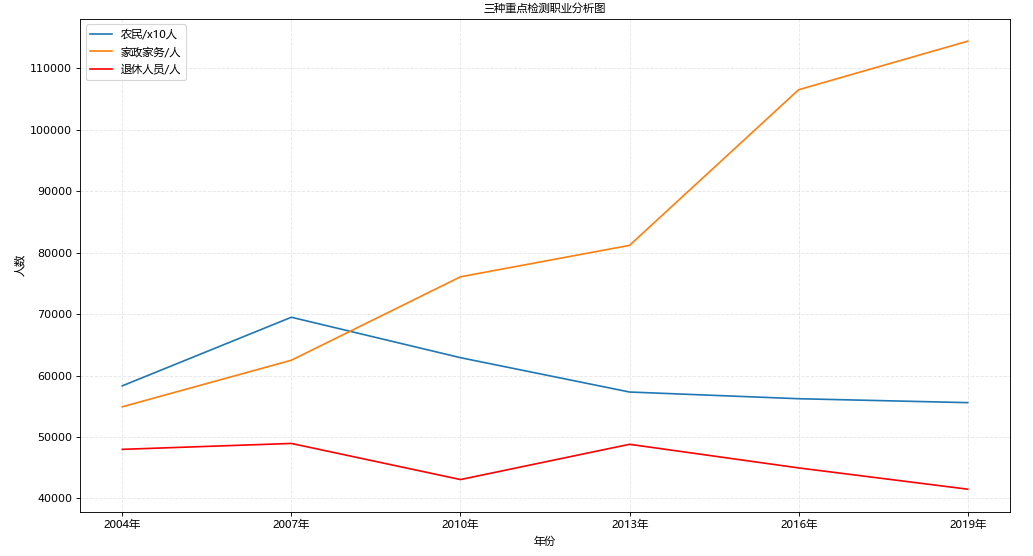
\includegraphics[width=\textwidth]{figures/sanrenf.png}
	   	\caption{问题一思维流程图}\label{lct}
	   \end{figure}

   
	    \subsection{模型的建立}
	    \subsubsection{经典旅行商模型}
	    分析问题一,由于大型运输车的行驶速度固定,优化行驶路径使得运输车行驶路程最短时,即可求得最小运输时间。遍历路径可表示为二维有限序列如下:
	     \begin{gather}
	    P_n=[p_{1},p_{2},\cdots,p_{i},\cdots,p_{19}]
	    \end{gather}
	    其中$p_{i}(1\leqslant i \leqslant 19 ,i\in Z)$表示处运输起点外的的仓库坐标,且对于$\forall i \neq j$都有$p_i \neq p_j $。任意两坐标点$p_i(x_i,y_i)$,$p_j(x_j,y_j)$间的曼哈顿距离可表示为:
	     \begin{gather}
	     d(p_i,p_j)=\left | x_i-x_j \right |+\left | y_i-y_j \right |
	     \end{gather}
	    将运输车行驶路程作为优化目标即可得到目标函数如下:
	    \begin{gather}
	    f(P_n)=d(p_0,p_{1})+d(p_0,p_{19})+\sum_{i=1}^{18}d(p_i,p_{i+1})
	    \end{gather}
	    即可得到整体优化模型如下:
	    \begin{gather}
	    f(P_n)=d(p_0,p_{1})+d(p_0,p_{19})+\sum_{i=1}^{18}d(p_i,p_{i+1})\\
	    \left\{\begin{matrix}1\leqslant i \leqslant 19 ,i\in Z
	    \\ \forall i \neq j,p_i \neq p_j 
	    \end{matrix}\right.
        \end{gather}
        \subsection{模型的求解}
        \subsubsection{遗传算法}
        \paragraph{初始化编码}
        对于表示为二维有限序列的遍历路径$P_n$,对其进行整数编码为
        \begin{gather}
        A_n=[a_{n1},a_{n2},\cdots,a_{ni},\cdots,a_{n19}], \\
        1\leqslant a_i \leqslant 19 ,i\in Z ;\forall i, \neq j\Rightarrow p_i \neq p_j 
        \end{gather}
        定义$A_n$为解序列$P_{n}$,其中$a_{ni}$表式对应仓库的访问顺序,例如 $a{i}=7$表示第$i$次访问7号仓库。即随机生成初始解集$A=\left \{A_n\right \}$其中$n=1,2,\cdots,w$,w为的种群容量。
        \paragraph{交叉}
        在原染色解集 $\left \{ A_n \right \}$中的染色体按照随机顺序配对,按照以下的方式交叉(补全),生成交叉解集$\left \{H_n\right \}$
         \begin{figure}[H]
        	\centering
        	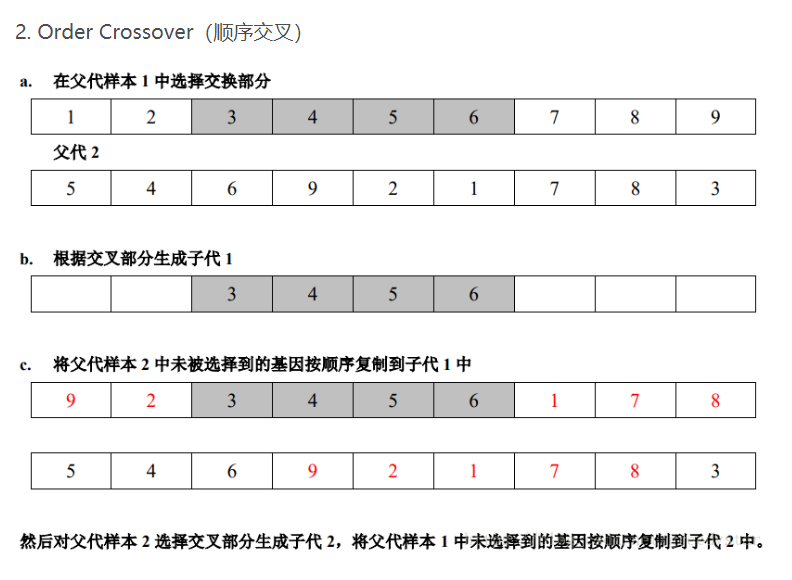
\includegraphics[width=\textwidth]{figures/2121.png}
        	\caption{交叉}\label{lct}
        \end{figure}
         \paragraph{变异}
         鉴于序列式染色体的特殊性,为了在变异阶段内尽可能不破坏原有的基因段,采取改良圈算法的思路进行变异操作。即在染色体$A$中随机选取$a_{i}$与$a_{j}(1\leqslant i<j\leqslant j )$,颠倒$a_{ni}$与$a_{nj}$间顺序的顺序,即:
          \begin{gather}
          M=[a_{1},\cdots,a_{i},a_{j-1},a_{j-2},\cdots,a_{i+1},a_{i},\cdots,a_{19}]
          \end{gather}
          $M$为染色体$A$对应的变异染色体,对于每个染色体$A_n$,都设定相同的变异概率$\gamma$去执行上述的变异操作。 
         \subsubsection{动态赌轮}
         将第g代的染色体与其交叉和变异产生的子代并入同一解集$G_g=\left \{A,H,M\right \}$。$k$表示原解集$A$,交叉解集$H$和变异解集$M$中解的数量之和,即为$G_g$中的解的数目。设置$G_g$第$i$个解$G_g(i)$被选择进入下一代的概率为:
         \begin{gather}
          P(G_{g}(i))=\frac{wf^{-g/\gamma }(G_{g}(i))}{\sum_{j=1}^{k}f^{-g/\gamma }(G_{g}(j))}
         \end{gather}
         $f^{-g/\gamma }(G_{g}(i))$为$G_{g}(i)$对应的目标函数值,即为$G_{g}(i)$对应的适应度。其中参数$\gamma$为衰减系数,$w$为种群容量。即适应度值相对较小的解保留概率将逐渐增大,
         即算法初始阶段将保留丰富度尽可能多的解,而愈到算法后期,策略就越接近于精英策略,加快算法的收敛速度,即有:
           \begin{gather}
           \lim_{g\rightarrow \infty } P(G_{g}(min))=\lim_{g\rightarrow \infty }\frac{wf^{-g/\gamma }(min)}{\sum_{j=1}^{k}f^{-g/\gamma }(G_{g}(j))}\rightarrow 1
         \end{gather}
         该式表明当迭代次数$g$足够大时,选择策略将趋近于为精英策略,将加速算法的收敛。
         
         
         
	  \section{问题二模型的建立与求解}
	  \subsection{问题描述与分析}
	  问题二要求设计小型运输车的调度方案,从而使得总体调度效率最高。我们将时间限制设置为约束,着重优化方案的经济效率。在问题一的基础上重新建立模型,鉴于第二问的决策变量是多段序列的和,我们设计了插板编码对决策变量进行编码,并基于问题一中的动态赌轮遗传算法以运输总成本为目标进行优化。
	  \subsection{模型的建立}
	  \subsubsection{带约束的多旅行商模型}
	  当雇佣$b$辆小型运输车时,总决策序列可表示为
	  \begin{gather}
	  P_n=\left \{[p_{1},p_{2}]_1,[\cdots,p_{i}]_j,[\cdots]_{b-1},[p_{19}]_b\right \}
	  \end{gather}
	  即将类似于模型一中的坐标序列分割为多段,每一段分别由一辆小型运输车单独完成,定义
	  \begin{gather}
	  B_j=
	  \end{gather}
      \subsection{模型的求解}

 
  
  
  
  \section{灵敏度分析}
  
  
  
  \section{模型的评价}
  \subsection{模型的优点}
  \begin{itemize}                                             
  	\item [(1)] 利用马尔可夫模型改进后的灰度预测值与实际值拟合度更高,波动性保持一致,预测的效果更好。
  	\item [(2)] 针对支持向量回归参数选取,利用灰色关联度筛选合适指标,相较于主观选取指标具有客观性、严谨性。	
  \end{itemize}
  \subsection{模型的缺点}
  
  问题一、二中的灰色预测模型只能做短期预测,并不适用于长期预测。
  \subsection{模型改进}
  
  可以通过序列最小优化算法(Sequential Minimal Optimization,SMO)作为样本的训练算法,进而建立序列最小优化支持向量回归模型,从而减小算法复杂度,提高算法的求解速度。
  
  
  
 
	\newpage	%换页符
	%%参考文献
	%\begin{thebibliography}{9}%宽度9
	% \setlength{\itemsep}{-2mm}
	\nocite{*}		%排版未引用的参考文献
%\bibliography{wenxian.bib}
%	%参考文献添加到wenxian.bib里,再引用
%	
\begin{thebibliography}{9}%宽度9
	\bibitem{bib:one}张斯嘉, 郭建胜, 钟夫, 等. 基于蝙蝠算法的多目标战备物资调运决策优化[J]. 火力与指挥控制, 2016, 41(1): 58-61.
	\bibitem{bib:2}李健, 张文文, 白晓昀, 等. 基于系统动力学的应急物资调运速度影响因素研究[J]. 系统工程理论与实践, 2015, 35(3): 661-670.	
	\bibitem{3}Wang J, Ersoy O K, He M, et al. Multi-offspring genetic algorithm and its application to the traveling salesman problem[J]. Applied Soft Computing, 2016, 43: 415-423.
	\bibitem{4}陶丽华, 马振楠, 史朋涛, 等. 基于 TSP 问题的动态蚁群遗传算法[J]. 机械设计与制造, 2019 (12): 39.
\end{thebibliography}

	\newpage
	%附录
	\appendix %%附录

\section{模型的代码实现}

\subsection{数据可视化--python源代码}
\begin{lstlisting}[language=python]

_xtick_labels = ["{}年".format(int(i)) for i in x]
plt.xticks(x, _xtick_labels, fontproperties=my_font)
# plt.yticks(range(0, 9))

# 绘制网格
plt.grid(alpha=0.3, linestyle="--")  # alpha为透明度 0-1
plt.title("三种重点检测职业分析图", fontproperties=my_font)
plt.xlabel("年份", fontproperties=my_font)
plt.ylabel("患病人数", fontproperties=my_font)
# 标注图例
plt.legend(prop=my_font, loc=0)
plt.show()
\end{lstlisting}


\end{document}